\chapter{Background}
\label{chapter:background}
\section{Call and Put Options}
As stated before, call and put options enable their buyer to buy and sell the underlying stock at the maturity for the fixed strike price.
In the case of a call option, if at the maturity the price of my asset is greater than the strike, I can buy it for the latter and immediately sell it for its higher market price. Thus, the payoff of my option would be the difference of these two values. On the other hand, if the price of the asset decreases past the strike at the maturity, I should let my option expire, since I can buy the asset for the lower market price rather than the higher strike. In this case, the payoff of the option would be zero.
The same reasoning can be made for put type options.
The payoff function of these two types of options can then simply be deduced as
\begin{equation}\label{callput}
\begin{split}
&\text{Payoff}_\text{call}=\max\left(S(T)-K,0\right);\\
&\text{Payoff}_\text{put}=\max\left(K-S(T),0\right),
\end{split}
\end{equation}
\noindent where $K$ is the strike price and $S(T)$ is the asset price, $S(t)$, at the maturity, $T$. These functions are represented in \autoref{fig:Payoff}.

\begin{figure}[!htb]
    \centering
      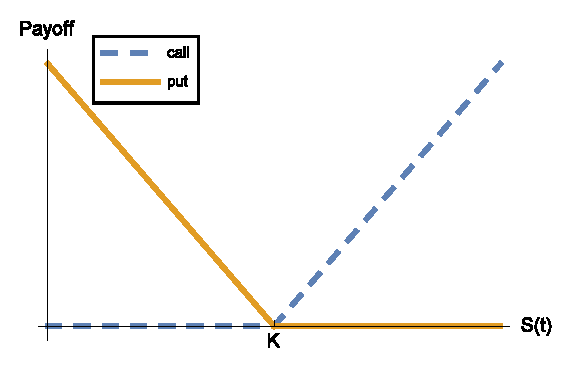
\includegraphics[width=.5\columnwidth]{Payoff.eps}
      \caption{Payoff functions of \emph{call} and \emph{put options}.}\label{fig:Payoff}
    \end{figure}
    
\section{Black-Scholes-Merton Formulae}
\label{section:Black-Scholes-Merton Formulae}
Due to their high importance, options have been studied in great detail in the past.
Probably the most important result in this field came from Fischer Black, Myron Scholes and Robert Merton, who developed a mathematical model to price options~\cite{Scholes} - the famous Black-Scholes-Merton model - still in use in present days~\cite{Wilmott}. The last two actually earned the 1997 Nobel prize in Economics for this development.

This model states that the price of an European call or put option, whose underlying asset is a stock, follows the partial differential equation (PDE)

\begin{equation}\label{BS2}
\pdv{V}{t}+\frac{1}{2}\sigma^2S^2\pdv{^2V}{S^2}+rS\pdv{V}{S}-rV=0,
\end{equation}

\noindent where $V$ is the price of the option, $S$ is the price of the underlying stock, $r$ is the risk-free interest rate and $\sigma$ is the stock price volatility.

The risk-free interest rate, $r$, is the interest an investor would receive from a risk-free investment. An investor should never invest in risky products whose expected return is lower than this interest, since there's the alternative of investing without risk. In general, this rate changes slightly with time, but Black \textit{et al.} assumed, in their original model, that it remains constant throghout the option duration. Some later developments dealt with this shortcoming, but because option prices do not significantly depend on this value~\cite{Wilmott}, in the remainder of this thesis we shall assume it is constant and known.

Finally, the volatility, $\sigma$, is a measure of uncertainty and will be studied in more detail in section \ref{section:volatility}.

One important assumption of this model is that stock prices follow a Geometric Brownian Motion (GBM), defined as
\begin{equation}\label{GBM}
dS(t)=rS(t)dt+\sigma S(t)dW(t),
\end{equation}
\noindent with $\{W(t),\ t>0\}$ defining a one-dimensional Brownian motion.


Pricing options is fairly straightforward - we simply need to solve the PDE in eq. \eqref{BS2} in a similar fashion to the initial value problem for the diffusion equation~\cite{Dilao}.
The results published in the original article by Black \textit{et al.} state that, at time $t$, call and put options can be valued as
\begin{equation}\label{callputBS}
\begin{split}
&C(S(t),t)=N(d_1)S(t)-N(d_2)Ke^{-r(T-t)};\\
&P(S(t),t)=-N(-d_1)S(t)+N(-d_2)Ke^{-r(T-t)},
\end{split}
\end{equation}
\noindent where $N(\cdot)$ is the cumulative distribution function of the standard normal distribution, $T$ is the maturity time, and $d_1$, $d_2$ are given by
\begin{equation}\label{d1d2}
\begin{split}
&d_1=\frac{1}{\sigma\sqrt{T-t}}\left[\ln\left(\frac{S_t}{K}\right)+\left(r+\frac{\sigma^2}{2}\right)(T - t)\right];\\
&d_2=d_1-\sigma\sqrt{T-t}.\\
\end{split}
\end{equation}



From eq. \eqref{callputBS} we can derive a relationship between $C(S,t)$ and $P(S,t)$, known as the \emph{put-call parity}
\begin{equation}
C(S(t),t)=S(t)-Ke^{-r(T-t)}+P(S(t),t).
\end{equation}
\noindent Because of this duality, we can always obtain the prices of put options from call options with the same underlying asset, maturity and strike. For this reason, unless otherwise stated, all options will be assumed calls in the following sections.


\section{Volatility}
\label{section:volatility}
Volatility is a measure of the uncertainty of future stock prices changes. In other words, a high volatility will lead to great future fluctuations in the stock price, whereas a stock with low volatility is more stable.

Of all the parameters in the Black-Scholes formula, \eqref{BS2}, volatility is the only one we can't easily observe from market data.
Furthermore, unlike the interest rate, volatility has a great impact on the behavior of stock prices and consequently on the price of options.
These two factors make volatility one of the most studied subjects in option pricing.



It should be noted that there are several types of volatility, depending on what is being measured. Some of these types will be approached in the next subsections.

\subsection{Implied Volatility}
\label{section:impliedvolatility}
The \emph{implied volatility} can be described as the value of stock price volatility that, when input into the Black-Scholes pricer in eq. \eqref{callputBS}, outputs a value equal to the market price of a given option.
In other words, it would be the stock volatility that the seller/buyer of the option assumed when pricing it (given that the Black-Scholes model was used).

Because eq. \eqref{callputBS} is not invertible, we need to use some numerical method (e.g Newton's method) to find the solution to the equation
\begin{equation}
C(\sigma_{imp},S(t),t)-\overline{C}=0,
\end{equation}
\noindent where $C(\sigma_{imp},\cdot)$ corresponds to the solution of eq. \eqref{callputBS} using the implied volatility $\sigma_{imp}$ and $\overline{C}$ is the price of the option observed at the market.

We can obtain the implied volatility of an option from its price or the price from its implied volatility, because eq. \eqref{callputBS} is monotonic in the volatility. This duality is so fundamental that exchanges sometimes sell their options providing only the implied volatility instead of the price~\citep{Wilmott}.

One interesting property of implied volatility is that, in the real-world, it varies with the strike price and maturity. In principle, if investors really used the Black-Scholes model to price their options, two options with the same underlying asset should have the same implied volatility, despite their strike prices or maturities.
However, when observing market data, this is not the case. The observed implied volatilities form two possible shapes in a scatter plot, known as \emph{smile} and \emph{skew}.
An implied volatility smile shows greater $\sigma_{imp}$ for options with strikes different from the current stock price and the minimum where the strike equals the stock price. A skew, on the other hand, only shows greater $\sigma_{imp}$ in one of the directions (i.e. for strikes either higher or lower than the current stock price). You can observe both these phenomena in \autoref{fig:smileskew}.
We can therefore conclude that options with strikes different from the current stock price are overpriced.
The reason behind this odd market behavior is the simple demand-supply rule~\citep{Wilmott}. On the one hand, some investors are risk-averse and want to hedge their losses in case of a market crash (as explained in subsection \ref{subsection:why options are important}). They don't mind paying a higher price for an option if this means they would be safe from crashes. For this reason, the prices of low strike (call) options increase which drives their implied volatility up. On the other hand, some other investors are risk-seekers and want to take advantage of possible sudden price increases, buying the stocks for lower prices. They don't mind paying higher prices for the options and this drives the prices of high strike options (and, consequently, their implied volatility) up.
    
    
\begin{figure}[!htb]
  \begin{subfigmatrix}{2}
    \subfigure[Smile]{\includegraphics[height=0.20\linewidth]{Smile.png}}
    \subfigure[Skew]{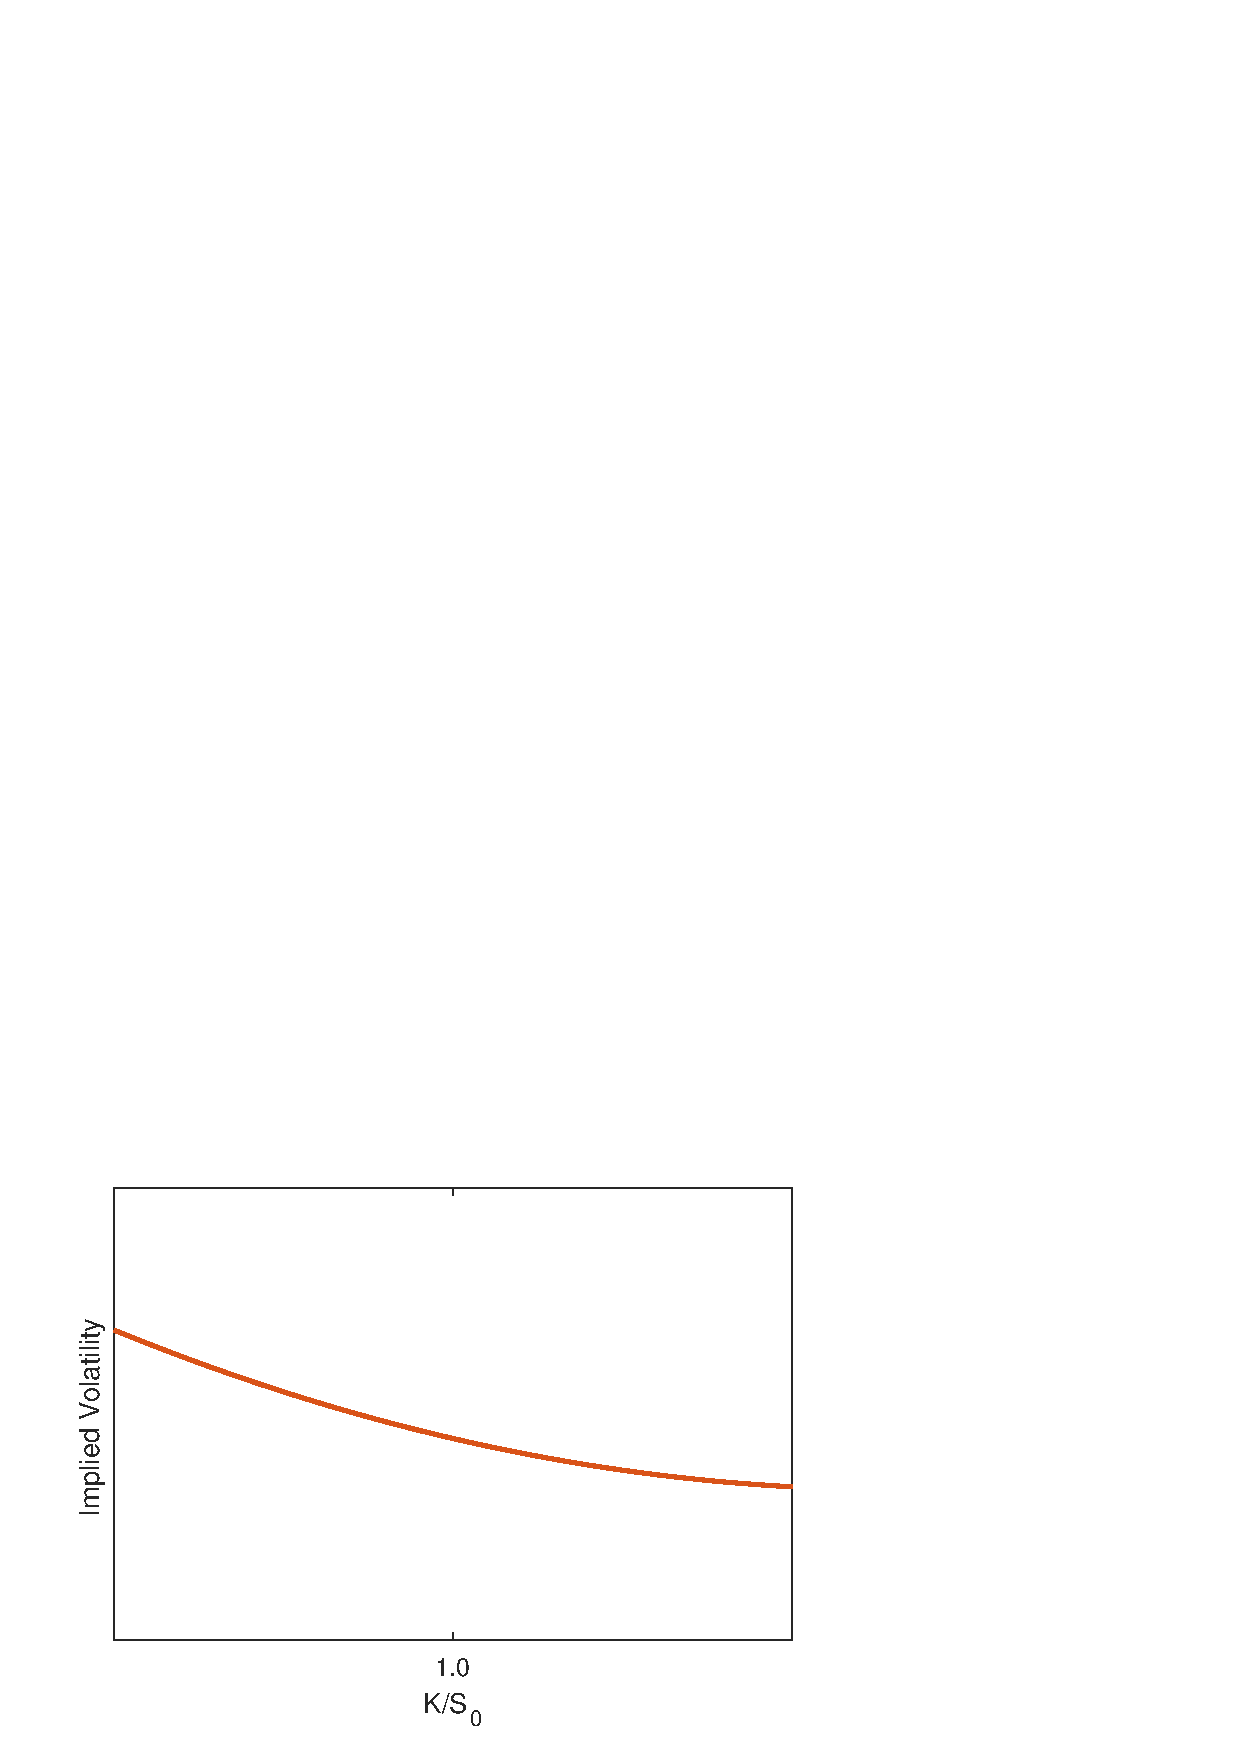
\includegraphics[height=0.20\linewidth]{Skew.png}}
  \end{subfigmatrix}
  \caption{Example of an implied volatility smile and skew.\hl{source=Hull}}
  \label{fig:smileskew}
\end{figure}

\subsection{Local Volatility}
\label{subsection:localvolatility}
In their original work, Black \textit{et al.} assumed that volatility is constant throughout the whole contract. From market data, it can be clearly seen that this is not the case. There may be times where new information reaches the market and trading increases, driving volatility up. The opposite is also true.

The model in eq. \eqref{callputBS} is clearly not enough to truly grasp real-world trading. We should have a model where volatility is dynamic, measuring the amount of randomness in the stock price at any given time.
The geometric Brownian motion from eq. \ref{GBM} would thus become
\begin{equation*}
dS(t)=rS(t)dt+\sigma(t) S(t)dW(t),
\end{equation*}
\noindent where $\sigma(t)$ is now some function of time.


However, as we saw in subsection \ref{section:impliedvolatility} for implied volatility, the market's view of volatility also varies with the strike price. A simple dynamic volatility model is thus unsufficient. The local volatility should then be a function of both time and strike price. We are left with a new GBM, given by
\begin{equation}\label{GBM2}
dS(t)=rS(t)dt+\sigma(K,t) S(t)dW(t),
\end{equation}
\noindent where $\sigma(K,t)$ depends now on $K$ and $t$.

The local volatility function is very difficult to measure. Some models have been proposed to model it. We shall approach them in section \ref{section:Dupire}.


\section{Dupire's Formula}
\label{section:Dupire}

\iffalse
Because the stock price depends on a Brownian motion process, it follows that it is not differentiable. For this reason, it's impossible to exactly simulate such a process. An approximation is possible, however, using discrete jumps of length $\Delta t$ and using the Brownian motion property $W(t)\sim \sqrt{t}N(0,1)$~\cite{Mikosch}, with $N(0,1)$ being a normal distribution with 0 expected value and 1 variance.
We can then simply discretize eq. \eqref{BS} into
\begin{equation}
S(t+\Delta t)=S(t)+rS(t)\Delta t+\sqrt{\Delta t}\sigma S(t)N(0,1),
\end{equation}
\noindent where $\Delta t$ corresponds to a given time step. An example of this discretization is illustrated in \autoref{fig:GBM} with the realization of three sample paths.

\begin{figure}[H]
    \centering
      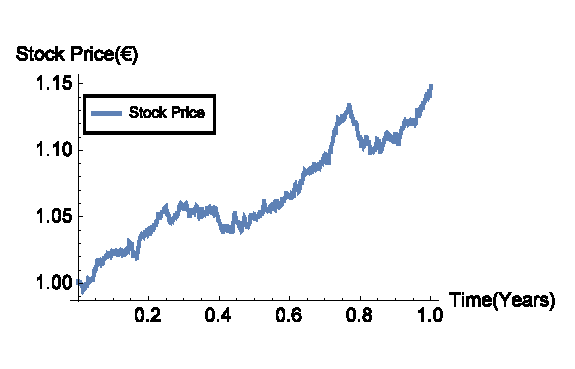
\includegraphics[width=0.9\columnwidth]{GBM.eps}
      \caption{Example of three GBM processes, using the parameters $r=\SI{0.06}{\per\year}$, $\sigma=0.05$, $S(0)=\SI{1}[\EUR]{}$ and time steps $\Delta t=10^{-3}\SI{}{\year}$.}\label{fig:GBM}
    \end{figure}
    
By simulating a large number of paths, some underlying tendencies might become apparent, which will prove useful in option pricing.


 American options, however, pose a much greater challenge.  Unlike European options, no analytic pricing model currently exists for this type of derivatives. Several numerical models have been proposed in the past in an attempt to solve this problem~\cite{Wilmott1,Hull}, such as the Longstaff-Schwartz algorithm~\citep{Longstaff}, which we shall approach in later sections of the present thesis.
\fi

%%%%%%%%%%%%%%%%%%%%%%%%%%%%%%%%%%%%%%%%%%%%%%%%%%%%%%%%%%%%%%%%%%%%%%%%
\section{Theoretical Overview}
\label{section:overview}


Some overview of the underlying theory about the topic...


%%%%%%%%%%%%%%%%%%%%%%%%%%%%%%%%%%%%%%%%%%%%%%%%%%%%%%%%%%%%%%%%%%%%%%%%
\section{Theoretical Model 1}
\label{section:theory1}

The research should be supported with a comprehensive list of references.
These should appear whenever necessary, in the limit, from the first to the last chapter.

A reference can be cited in any of the following ways:
%
\begin{itemize}
  \item Citation mode \#1 - \quad \cite{jameson:adjointns}
  \item Citation mode \#2 - \quad \citet{jameson:adjointns}
  \item Citation mode \#3 - \quad \citep{jameson:adjointns}
  \item Citation mode \#4 - \quad \citet*{jameson:adjointns}
  \item Citation mode \#5 - \quad \citep*{jameson:adjointns}
  \item Citation mode \#6 - \quad \citealt{jameson:adjointns}
  \item Citation mode \#7 - \quad \citealp{jameson:adjointns}
  \item Citation mode \#8 - \quad \citeauthor{jameson:adjointns}
  \item Citation mode \#9 - \quad \citeyear{jameson:adjointns}
  \item Citation mode \#10 - \quad \citeyearpar{jameson:adjointns}
\end{itemize}
%
Several citations can be made simultaneously as \citep{nocedal:opt,marta:ijcfd}. \\

This is often the default bibliography style adopted (numbers following the citation order), according to the options:\\
{\tt \textbackslash usepackage\{natbib\}} in file {\tt Thesis\_Preamble.tex},\\
{\tt \textbackslash bibliographystyle\{abbrvnat\}} in file {\tt Thesis.tex}.\\

Notice however that this style can be changed from numerical citation order to authors' last name with the options: \\
{\tt \textbackslash usepackage[numbers]\{natbib\}} in file {\tt Thesis\_Preamble.tex},\\
{\tt \textbackslash bibliographystyle\{abbrvunsrtnat\}} in file {\tt Thesis.tex}. \\

Multiple citations are compressed when using the {\tt sort\&compress} option when loading the {\tt natbib} package as {\tt \textbackslash usepackage[numbers,sort\&compress]\{natbib\}} in file {\tt Thesis\_Preamble.tex}, resulting in citations like \citep{marta:ijcfd1,marta:ijcfd2,marta:ijcfd3,marta:ijcfd4}.


%%%%%%%%%%%%%%%%%%%%%%%%%%%%%%%%%%%%%%%%%%%%%%%%%%%%%%%%%%%%%%%%%%%%%%%%
\section{Theoretical Model 2}
\label{section:theory2}

Other models...

